\documentclass{beamer}
\usetheme{Boadilla}

\usepackage[utf8]{inputenc}
\usepackage[ruled,vlined]{algorithm2e}
\usepackage{amsfonts}
\usepackage{hyperref}
\usepackage{multirow}
\usepackage{systeme}
\usepackage{tikz}
\usepackage{xcolor}

\usetikzlibrary{arrows.meta}
\hypersetup{
	colorlinks=true,
	linkcolor=blue,
	filecolor=magenta,      
	urlcolor=cyan,
}

\title{Introduction to Gaussian Processes}
\author{Noah J. Wichrowski}
\institute[JHU]{Johns Hopkins University}
\date{\today}

\newcommand{\N}{\mathbb{N}}
\newcommand{\Z}{\mathbb{Z}}
\newcommand{\R}{\mathbb{R}}
\newcommand{\ii}{\,\mathbf{i}}
\newcommand{\vect}[1]{\boldsymbol{#1}}

\newcommand{\E}[1]{\mathbb{E}\left[#1\right]}
\newcommand{\V}[1]{\mathbb{V}\left[#1\right]}
\newcommand{\iid}{\ensuremath{\stackrel{\text{iid}}{\sim}}}
\newcommand{\nml}{\mathcal{N}}

\newcommand{\argmaxx}{\mathop{\mathrm{argmax}}\limits}
\newcommand{\argminn}{\mathop{\mathrm{argmin}}\limits}
\newcommand{\lrarr}{\ensuremath{\leftrightarrow}}
\newcommand*\widefbox[1]{\fbox{\hspace{2em}#1\hspace{2em}}}
\providecommand{\norm}[1]{\lVert#1\rVert}
\renewcommand{\arraystretch}{1.25}
\let\emptyset\varnothing
\let\eps\varepsilon
\DeclareMathOperator{\Cov}{Cov}
\DeclareMathOperator{\diag}{diag}

\newcommand{\citeAY}[1]{
	\begin{flushright}
		{\footnotesize [#1]}
	\end{flushright}
}

\beamertemplatenavigationsymbolsempty
\setbeamertemplate{bibliography item}[triangle]
\begin{document}
	\begin{frame}
		\titlepage
	\end{frame}
	
	\begin{frame}
		\frametitle{Outline}
		\tableofcontents
	\end{frame}
	
	\section{Motivation}
	\begin{frame}
		\frametitle{Prelude: Linear Regression}
		\begin{itemize}
			\item Consider data $\mathcal{D}=\{(\vect{x}_i,y_i)\}_{i=1}^n\subset\R^d\times\R$.
			\item We want the weight vector $\vect{w}\in\R^d$ that yields the best linear fit $$f(\vect{x})=\vect{w}^\top\vect{x}\,.$$
			\item Let $X\in\R^{n\times d}$ be the design matrix, $\vect{y}\in\R^n$ the response vector.
			\item Then $\vect{\widehat{w}}=X^\dagger\vect{y}=(X^\top X)^{-1}X^\top\vect{y}$ minimizes the squared error: $$X^\dagger\vect{y}\in\argminn_{\vect{w}\in\R^d}=\norm{X\vect{w}-\vect{y}}_2^2\,.$$
		\end{itemize}
	\end{frame}

	\begin{frame}
		\frametitle{Linear Regression with Basis Functions}
		\begin{itemize}
			\item Consider data $\mathcal{D}=\{(\vect{x}_i,y_i)\}_{i=1}^n\subset\R^d\times\R$.
			\item For weight vector $\vect{w}\in\R^N$ and basis functions $\phi_j:\R^d\to\R$, $$f(\vect{x})=\vect{w}^\top\vect{\phi}(\vect{x})=\sum_{j=1}^Nw_j\phi_j(\vect{x})\,.$$
		\end{itemize}
		
		\begin{center}
			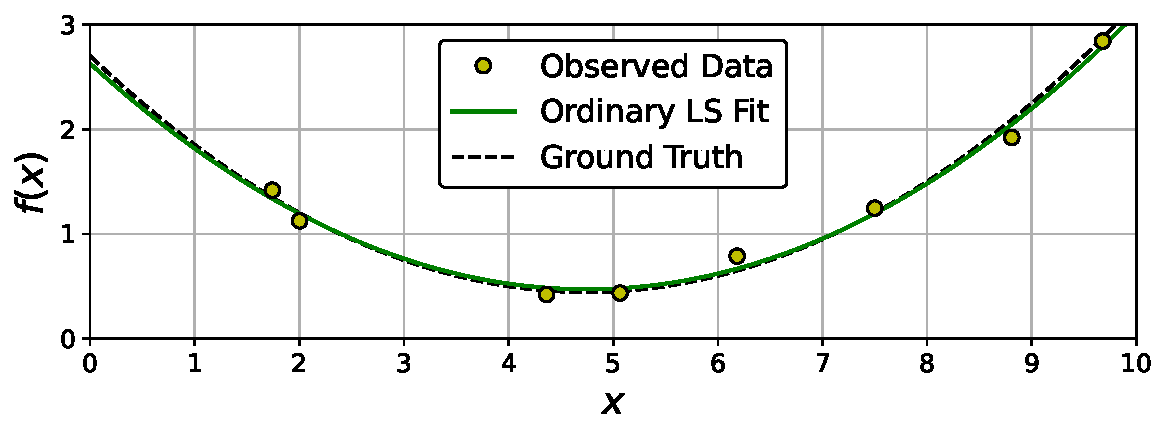
\includegraphics[scale=0.5]{figures/01b_ordinary_least_squares_wTrue.pdf}
		\end{center}
	\end{frame}
	
	\begin{frame}
		\frametitle{Bayesian Linear Regression}
		\begin{itemize}
			\item The standard linear model for ``frequentist'' regression is given by
			\begin{align*}
				f(\vect{x}) & =\vect{w}^\top\vect{x}\,,\\
				y_i & =f(\vect{x}_i)+\eps_i\,,\\
				\eps_i & \iid\nml(0,\sigma_\eps^2)\,.
			\end{align*}
			\item In a Bayesian framework, we have $\vect{y}\,|\,X,\vect{w}\sim\nml(X\vect{w},\sigma_\eps^2\,I)$.
			\item With prior $\vect{w}\sim\nml(\vect{0},\Sigma_p)$, the resulting posterior is
			\begin{align*}
				\vect{w}\,|\,X,\vect{y} & \sim\nml(\bar{\vect{w}},C)\,,\\
				C^{-1} & =\sigma_\eps^{-2}X^\top X+\Sigma_p^{-1}\,,\\
				\bar{\vect{w}} & =\sigma_\eps^{-2}CX^\top\vect{y}\,.
			\end{align*}
		\end{itemize}
		\citeAY{Rasmussen \& Williams, 2006}
	\end{frame}
	
	\begin{frame}
		\frametitle{Bayesian Linear Regression: Prediction}
		\begin{itemize}
			\item We can use the posterior on $\vect{w}$ to predict new observations.
			\item For a new input $\vect{x}_\star\in\R^d$,
			\begin{equation*}
				y_\star\,|\,\vect{x}_\star,X,\vect{y}\sim\nml(\bar{\vect{w}}^\top\vect{x}_\star,\;\vect{x}_\star^\top C\vect{x}_\star)\,.
			\end{equation*}
			\citeAY{Rasmussen \& Williams, 2006}
		\end{itemize}
		
		\begin{center}
			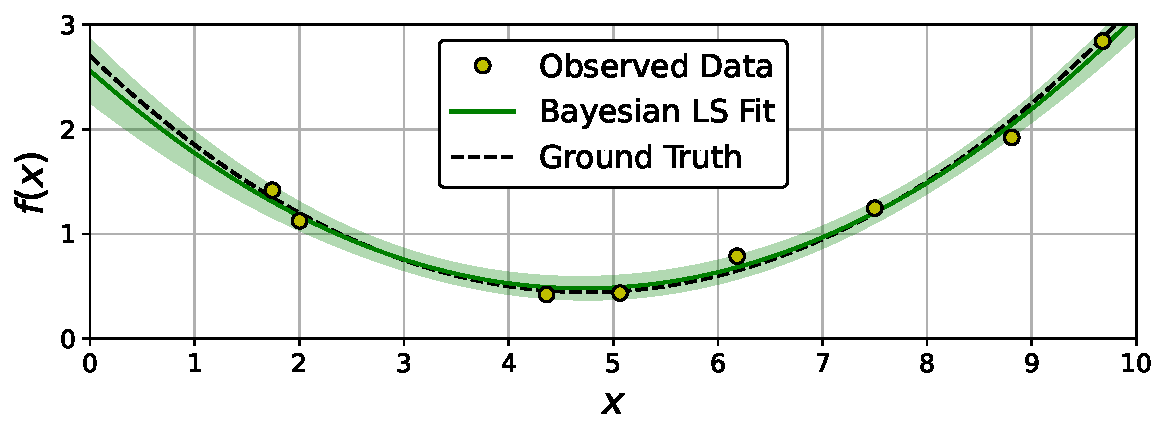
\includegraphics[scale=0.5]{figures/01c_bayesian_least_squares_wTrue.pdf} % \onslide<2> maybe?
		\end{center}
	\end{frame}
	
	\section{Gaussian Processes}
	\subsection{Definition and Sampling}
	\begin{frame}
		\frametitle{Gaussian Processes}
		\begin{definition}[Rasmussen and Williams, 2006]
			A Gaussian process (GP) is a collection of random variables $\{Y_{\vect{x}}\,|\,\vect{x}\in\mathcal{X}\}$, any finite number of which have a joint Gaussian distribution.
		\end{definition}
		\begin{itemize}
			\item The index set $\mathcal{X}$ is often an interval $T\subseteq\R$.
			\item A GP is completely specified by:
			\begin{itemize}
				\item mean function: $m(\vect{x})=\E{Y_{\vect{x}}}$
				\item covariance kernel: $k(\vect{x},\vect{x}')=\Cov[Y_{\vect{x}},Y_{\vect{x}'}]$
			\end{itemize}
		\end{itemize}
		\onslide<2>{
			\begin{example}[Pavliotis, 2014]
				Brownian Motion on $\R$:
				\begin{align*}
					m(t) & =0 & k(t,t') & =\min(t,t')
				\end{align*}
				Ornstein-Uhlenbeck Process:
				\begin{align*}
					m(t) & =x_0e^{-\alpha t} & k(t,t') & =\tfrac{1}{\alpha\beta}\left(e^{-\alpha|t-t'|}-e^{-\alpha(t+t')}\right)
				\end{align*}
			\end{example}
		}
	\end{frame}
	
	\begin{frame}
		\frametitle{Function-Space View of GPs}
		\begin{itemize}
			\item Any GP defines a distribution over functions $f:\mathcal{X}\to\R$: $$f(\vect{x}|\omega)=Y_{\vect{x}}(\omega)$$
			\item How do we sample $f\sim \mathcal{GP}\left[m(\cdot),k(\cdot,\cdot)\right]$?
			\begin{itemize}
				\item Choose $\mathcal{D}_X=\{\vect{x}_1,\ldots,\vect{x}_n\}$. % at which we want $f(\vect{x}_i)$.
				\item Compute $m_i=m(\vect{x}_i)$, $K_{ij}=k(\vect{x}_i,\vect{x}_j)$. % Compute mean vector $m_i=m(\vect{x}_i)$ and Gram matrix $K_{ij}=k(\vect{x}_i,\vect{x}_j)$.
				\item Draw $\vect{y}\sim\nml(\vect{m},K)$ and take $f(\vect{x}_i)=y_i$. % Draw a finite sample $\vect{y}\sim\nml(\vect{m},K)$. Take $f(\vect{x}_i)=y_i$.
			\end{itemize}
			\item Use conditional distributions to sample $y_\star=f(\vect{x}_\star)$ for $\vect{x}_\star\notin\mathcal{D}_X$:
			\begin{align*}
				\E{\vect{y}_\star|X_\star,X,\vect{y}} & =K(X_\star,X)K(X,X)^{-1}\vect{y}\\
				\Cov\left[\vect{y}_\star|X_\star,X,\vect{y}\right] & =K(X_\star,X_\star)-K(X_\star,X)K(X,X)^{-1}K(X,X_\star)
			\end{align*}
		\end{itemize}
		\citeAY{Rasmussen \& Williams, 2006}
	\end{frame}
	
	\begin{frame}
		\frametitle{Sampling from a GP}
		\begin{itemize}
			\item Prior distribution: $m(x)\equiv0$, $k(x,x')=\exp\!\left[-\tfrac{1}{2}(x-x')^2\right]$
			\item Can draw (discretized) functions from prior or posterior.
			\item Plotted points are entries from MVN vectors.
		\end{itemize}
		\begin{center}
			\includegraphics<1>[scale=0.5]{figures/02a_sample_from_prior.pdf}
			
			\includegraphics<2>[scale=0.5]{figures/02c_sample_from_posterior.pdf}
		\end{center}
	\end{frame}
	
	\subsection{Covariance Kernels}
	\begin{frame}
		\frametitle{Covariance Functions: Concepts}
		\begin{itemize}
			\item A kernel must be symmetric and positive semidefinite.
			\begin{itemize}
				\item For all $\vect{x},\vect{x}'\in\mathcal{X}$, $k(\vect{x},\vect{x}')=k(\vect{x}',\vect{x})$.
				\item Given measure $\mu$, for all $f\in L^2(\mathcal{X},\mu)$, 
			\end{itemize}
			$$\iint_{\mathcal{X}\times\mathcal{X}}k(\vect{x},\vect{x}')f(\vect{x})f(\vect{x}')\,d\mu(\vect{x})\,d\mu(\vect{x}')\geq0\,.$$
			\item We say $k$ is stationary if $k(\vect{x},\vect{x}')=g(\vect{x}-\vect{x}')$.
			\item We say $k$ is isotropic if $k(\vect{x},\vect{x}')=g(\norm{\vect{x}-\vect{x}'})$.
			\item Kernels can be added, multiplied, and scaled:
			\begin{equation*}
				k(\vect{x},\vect{x}') = c_1^2k_1(\vect{x},\vect{x}')+c_2^2k_2(\vect{x},\vect{x}')k_3(\vect{x},\vect{x}')\,.
			\end{equation*}
		\end{itemize}
		\citeAY{Duvenaud, 2014; Rasmussen \& Williams, 2006}
	\end{frame}

	\begin{frame}
		\frametitle{Continuity and Differentiability}
		\begin{definition}[Rasmussen and Williams, 2006]
			Let $f\sim \mathcal{GP}\left[m(\cdot),k(\cdot,\cdot)\right]$ be a Gaussian process on $\mathcal{X}\subseteq\R^d$. Then $f$ is continuous in mean square (CMS) at $\vect{x}_\star\in\mathcal{X}$ if $$\lim_{\vect{x}\to\vect{x}_\star}\E{|f(\vect{x})-f(\vect{x}_\star)|^2}=0\,.$$ We say that $f$ is mean-square differentiable (MSD) at $\vect{x}_\star$ with partial derivatives $\partial f(\vect{x}_\star)/\partial x_i$ if, for $i\in\{1,\ldots,d\}$, $$\lim_{h\to0}\E{\left(\frac{f(\vect{x}_\star+h\vect{e}_i)-f(\vect{x}_\star)}{h}-\frac{\partial f(\vect{x}_\star)}{\partial x_i}\right)^2}=0\,.$$
		\end{definition}
		\begin{itemize}
			\item GP with kernel $k$ is CMS at $\vect{x}_\star\in\mathcal{X}$ iff $k$ is continuous at $(\vect{x}_\star,\vect{x}_\star)$.
			\item A $2p$-order derivative of $k(\vect{x}_\star,\vect{x}_\star)$ ensures $f$ is MSD $p$ times at $\vect{x}_\star$.
		\end{itemize}
	\end{frame}

	\begin{frame}
		\frametitle{Covariance Kernels: Squared Exponential}
		\begin{equation*}
			k(\vect{x},\vect{x}')=\exp\left[-\frac{\norm{\vect{x}-\vect{x}'}^2}{2\ell^2}\right]\qquad\ell>0
		\end{equation*}
		\begin{itemize}
			\item Infinitely mean-square differentiable
			\item Often a limiting case of other kernel families
		\end{itemize}
		\begin{columns}
			\begin{column}{0.6\textwidth}
				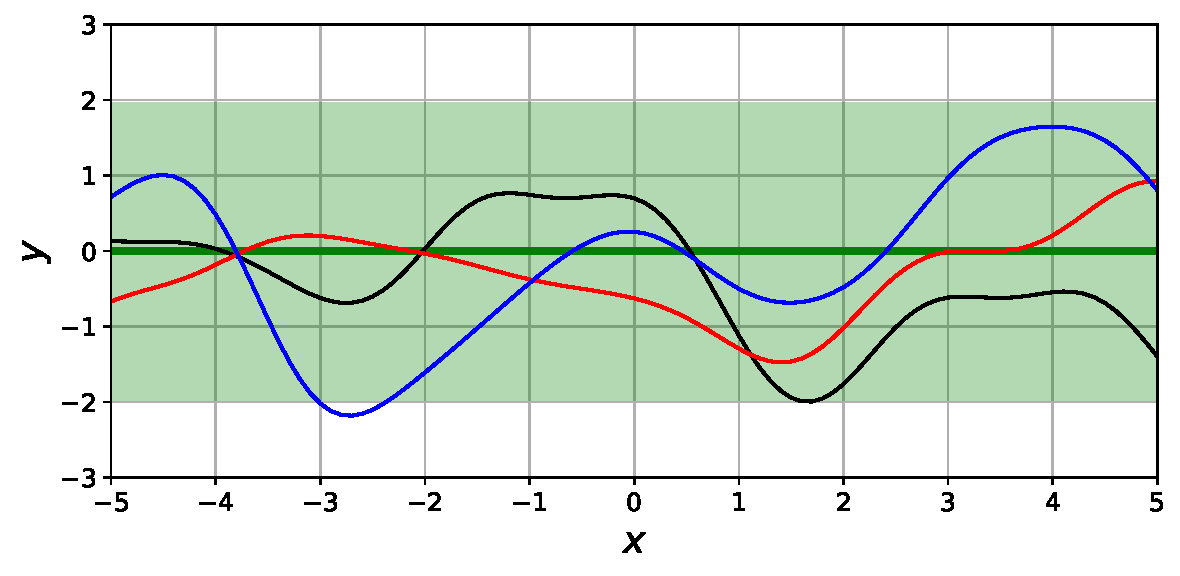
\includegraphics[width=\textwidth]{figures/03a_gaussian_sample.pdf}
			\end{column}
			\hfill
			\begin{column}{0.4\textwidth}
				\begin{center}
					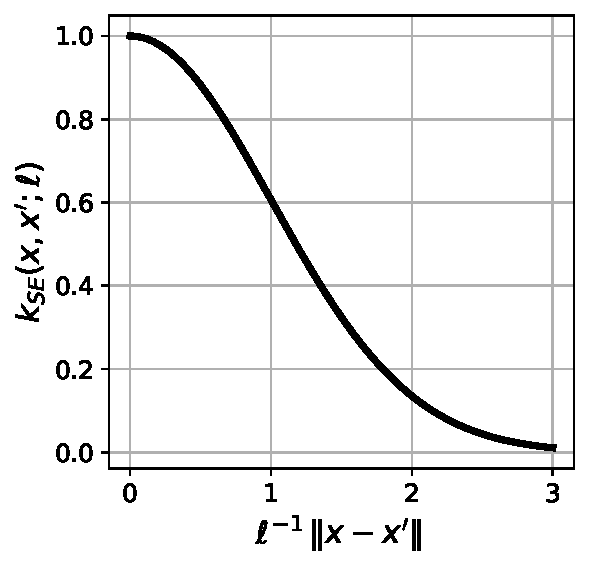
\includegraphics[width=0.8\textwidth]{figures/03a_gaussian.pdf}
				\end{center}
			\end{column}
		\end{columns}
	\end{frame}

	\begin{frame}
		\frametitle{Covariance Kernels: Periodic}
		\begin{equation*}
			k(\vect{x},\vect{x}')=\exp\left[-\frac{2\sin^2\left(\pi\norm{\vect{x}-\vect{x}'}/p\right)}{\ell^2}\right]\qquad\ell,p>0
		\end{equation*}
		%\begin{itemize}
		%	\item Infinitely mean-square differentiable
		%	\item Often a limiting case of other kernel families
		%\end{itemize}
		\begin{columns}
			\begin{column}{0.6\textwidth}
				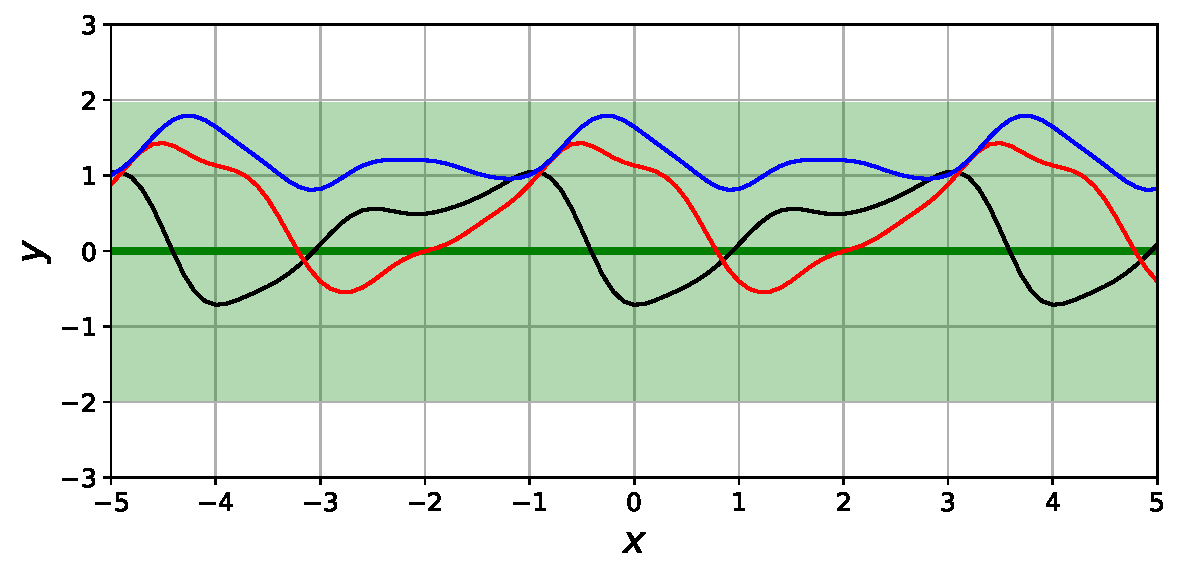
\includegraphics[width=\textwidth]{figures/03b_periodic_sample.pdf}
			\end{column}
			\hfill
			\begin{column}{0.4\textwidth}
				\begin{center}
					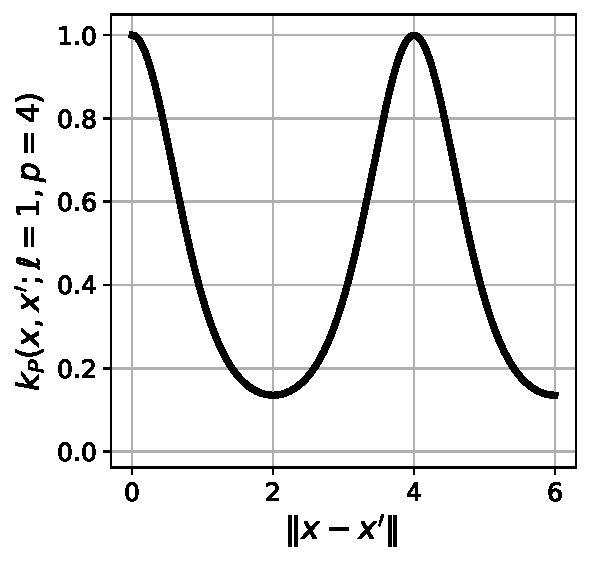
\includegraphics[width=0.8\textwidth]{figures/03b_periodic.pdf}
				\end{center}
			\end{column}
		\end{columns}
	\end{frame}

	\begin{frame}
		\frametitle{Covariance Kernels: Mat\'{e}rn}
		\begin{align*}
			k(\vect{x},\vect{x}') & =\frac{2^{1-\nu}}{\Gamma(\nu)}\left(\frac{r\sqrt{2\nu}}{\ell}\right)^\nu K_\nu\left(\frac{r\sqrt{2\nu}}{\ell}\right) & \ell,\nu & >0\\
			K_\nu(\cdot) & \text{ is a modified Bessel function} 
		\end{align*}
		\begin{columns}
			\begin{column}{0.6\textwidth}
				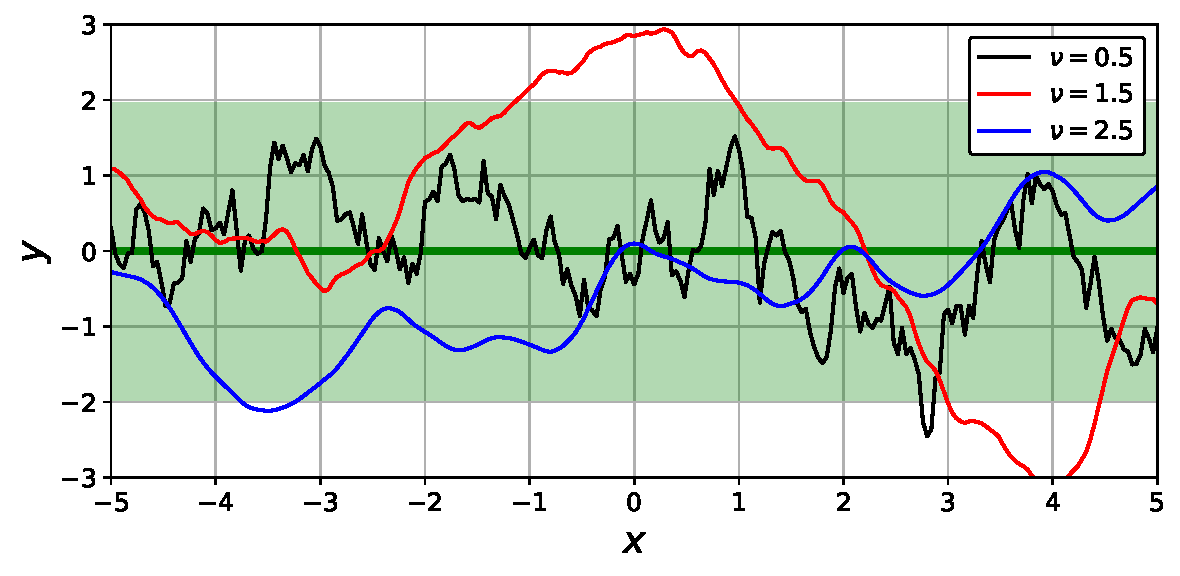
\includegraphics[width=\textwidth]{figures/03c_matern_sample.pdf}
			\end{column}
			\hfill
			\begin{column}{0.4\textwidth}
				\begin{center}
					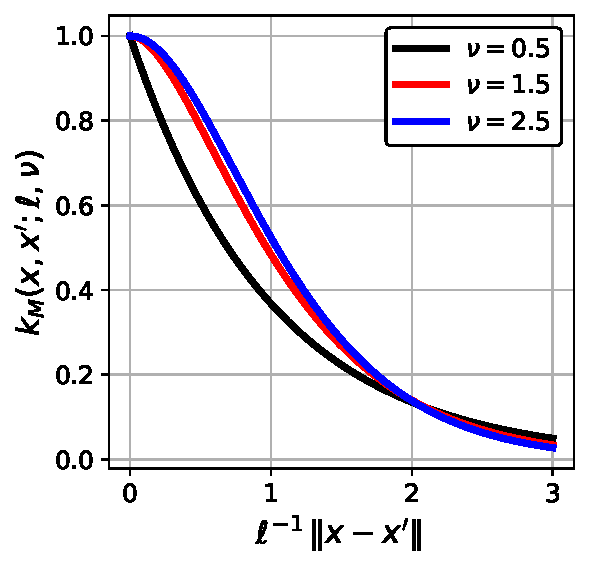
\includegraphics[width=0.8\textwidth]{figures/03c_matern.pdf}
				\end{center}
			\end{column}
		\end{columns}
	\end{frame}

	\begin{frame}
		\frametitle{Mat\'{e}rn Kernel Smoothness Parameter}
		\begin{itemize}
			\item Mean-square differentiable $\lceil\nu\rceil-1$ times.
			\item Reduces to squared exponential as $\nu\to\infty$.
			\item Simpler forms for $\nu+\tfrac{1}{2}\in\N$:
		\end{itemize}
		\begin{align*}
			{k_{1/2}(r)} & =\exp\left[-\frac{r}{\ell}\right] & k_{3/2}(r) & =\left(1+\frac{r\sqrt{3}}{\ell}\right)\exp\left[-\frac{r\sqrt{3}}{\ell}\right]\\
			& & k_{5/2}(r) & =\left(1+\frac{r\sqrt{5}}{\ell}+\frac{5r^2}{3\ell^2}\right)\exp\left[-\frac{r\sqrt{5}}{\ell}\right]
		\end{align*}
		\citeAY{Rasmussen \& Williams, 2006}
	\end{frame}

	\begin{frame}
		\frametitle{Generalizing Isotropic Kernels}
		\begin{itemize}
			\item Most common kernels are defined as $k(\vect{x},\vect{x}')=g(\norm{\vect{x}-\vect{x}'})$.
			\item What if some directions are more important than others?
			\begin{equation*}
				k(\vect{x},\vect{x}')=g\left(\sum_{i=1}^d\frac{|x_i-x_i'|}{\ell_i}\right)
			\end{equation*}
			\item For interactions among directions, use a Mahalanobis metric, \emph{e.g.},
			\begin{equation*}
				k(\vect{x},\vect{x}')=\exp\left[-(\vect{x}-\vect{x}')^\top M^{-1}(\vect{x}-\vect{x}')\right]\,,
			\end{equation*}
			with $M$ symmetric, positive definite.
		\end{itemize}
	\end{frame}
	
	\subsection{Regression with GPs}
	\begin{frame}
		\frametitle{Fitting GPs to Data}
		\begin{itemize}
			\item Consider data $\mathcal{D}=\{(\vect{x}_i,y_i)\}_{i=1}^n\subset\R^d\times\R$.
			\item Recall the prediction for $y_\star=f(\vect{x}_\star)$ at $\vect{x}_\star\notin\mathcal{D}_X$:
			\begin{align*}
				\E{\vect{y}_\star|X_\star,X,\vect{y}} & =K(X_\star,X)K(X,X)^{-1}\vect{y}\\
				\Cov\left[\vect{y}_\star|X_\star,X,\vect{y}\right] & =K(X_\star,X_\star)-K(X_\star,X)K(X,X)^{-1}K(X,X_\star)
			\end{align*}
			\item Must account for measurement noise when choosing a model.
			\item Given $\mathcal{D}$, the GPR model is specified by our choice of kernel.
		\end{itemize}
		\citeAY{Goldberg \emph{et al.}, 1997; Rasmussen \& Williams, 2006}
	\end{frame}
	
	%%% TO DO %%%
	%\begin{frame}
	%	\frametitle{Surrogate as Sum of Basis Functions}
	%	\begin{itemize}
	%		\item ...
	%	\end{itemize}
	%\end{frame}
	
	\begin{frame}
		\frametitle{Model Selection}
		\begin{itemize}
			\item GP Regression requires:
			\begin{itemize}
				\item Selecting a kernel function (model).
				\item Tuning hyperparameters $\vect{\theta}\in\R^p$.
			\end{itemize}
			\item The log-marginal likelihood is
			\begin{align*}
				\log p(\vect{y}\,|\,X,\vect{\theta}) & =-\tfrac{1}{2}\,\vect{y}^\top K_{\vect{\theta}}^{-1}\vect{y}-\tfrac{1}{2}\log|K_{\vect{\theta}}|-\tfrac{n}{2}\log(2\pi)\,,\\
				K_{\vect{\theta}} & =K(X,X;\vect{\theta})+N(\vect{\theta})\,,
			\end{align*}
			where $N(\vect{\theta})$ models noise in outputs, $y_i=f(\vect{x}_i)+\eps_i$.
			\item Cross-validation is also possible.
			\begin{itemize}
				\item Block matrix inversion speeds up prediction.
				\item Loss minimization requires expensive derivatives.
			\end{itemize}
		\end{itemize}
		\citeAY{Rasmussen \& Williams, 2006}
	\end{frame}
	
	%%% TO DO %%%
	%\begin{frame}
	%	\frametitle{(Error Measurement) (MSLL)}
	%	\begin{itemize}
	%		\item ...
	%	\end{itemize}
	%	\citeAY{Rasmussen \& Williams, 2006}
	%\end{frame}
	
	\begin{frame}
		\frametitle{Model Selection: An Illustration}
		\begin{itemize}
			\item Observed outputs are corrupted by iid $\nml(0,0.3^2)$ noise.
			\only<1>{
				\item Assuming outputs are noiseless: length scale $\ell=0.0972$
			}\only<2>{
				\item Including noise-level hyperparmater: length scale $\ell=1.42$
			}
		\end{itemize}
		\vspace{2mm}
		
		\begin{center}
			\includegraphics<1>[scale=0.5]{figures/04a_regression_noiseless.pdf}
			
			\includegraphics<2>[scale=0.5]{figures/04b_regression_optimal.pdf}
		\end{center}
	\end{frame}

	\section{GP Models}
	\subsection{Noisy Observations}
	\begin{frame}
		\frametitle{Dealing with Noisy Outputs}
		\begin{itemize}
			\item Often, we can only observe $y_i=f(\vect{x}_i)+\eps_i$.
			\item Standard approach: assume independent $\eps_i\sim\nml(0,\sigma_\eps^2)$
			\item Predictive distribution is given by
		\end{itemize}
		\begin{align*}
			\E{\vect{y}_\star|X_\star,X,\vect{y}} & =K(X_\star,X)K_{\vect{y}}^{-1}\vect{y}\\
			\Cov\left[\vect{y}_\star|X_\star,X,\vect{y}\right] & =K_{\star}-K(X_\star,X)K_{\vect{y}}^{-1}K(X,X_\star)\\
			K_{\vect{y}} & =K(X,X)+\sigma_\eps^2\,I\\
			K_{\star} & =K(X_\star,X_\star)+\sigma_\eps^2\,I
		\end{align*}
	\end{frame}

	\begin{frame}
		\frametitle{Uncertainty vs. Variability}
		\begin{itemize}
			\item Often wrongly used as synonyms.
			\begin{itemize}
				\item Uncertainty: Lack of knowledge of a deterministic quantity
				\item Variability: Differences in nominally interchangeable objects
			\end{itemize}
			\item Distinct, but intertwined, concepts.
			\begin{itemize}
				\item Uncertainty is quantified in probabilistic terms.
				\item Variability is expressed in the language of statistics.
			\end{itemize}
			\item Two main classes of uncertainty:
			\begin{itemize}
				\item Aleatoric: difference in outcomes from repeated experiments
				\item Epistemic: imprecise results from incomplete information
			\end{itemize}
		\end{itemize}
		\citeAY{Begg \emph{et al.}, 2014; Der Kiureghian \& Ditlevsen, 2009}
	\end{frame}
	
	\begin{frame}
		\frametitle{An Important Distinction}
		\begin{center}
			Consider independent variables $X_i\iid\nml(0,1)$.
		\end{center}
		\begin{columns}
			\begin{column}{0.5\textwidth}
				\begin{center}
					\underline{Estimate the Mean}
				\end{center}
			\end{column}
			\begin{column}{0.5\textwidth}
				\begin{center}
					\underline{Predict the Next Value}
				\end{center}
			\end{column}
		\end{columns}
		\vspace{1mm}
		\begin{columns}
			\begin{column}{0.5\textwidth}
				\begin{equation*}
					\V{\bar{X}_n}=\V{\frac{1}{n}\sum_{i=1}^nX_i}=\frac{1}{n}\to0
				\end{equation*}
			\end{column}
			\begin{column}{0.5\textwidth}
				\begin{equation*}
					\V{X_{n+1}}=1\hspace{2mm}\forall\,n\in\N
				\end{equation*}
			\end{column}
		\end{columns}
		\begin{center}
			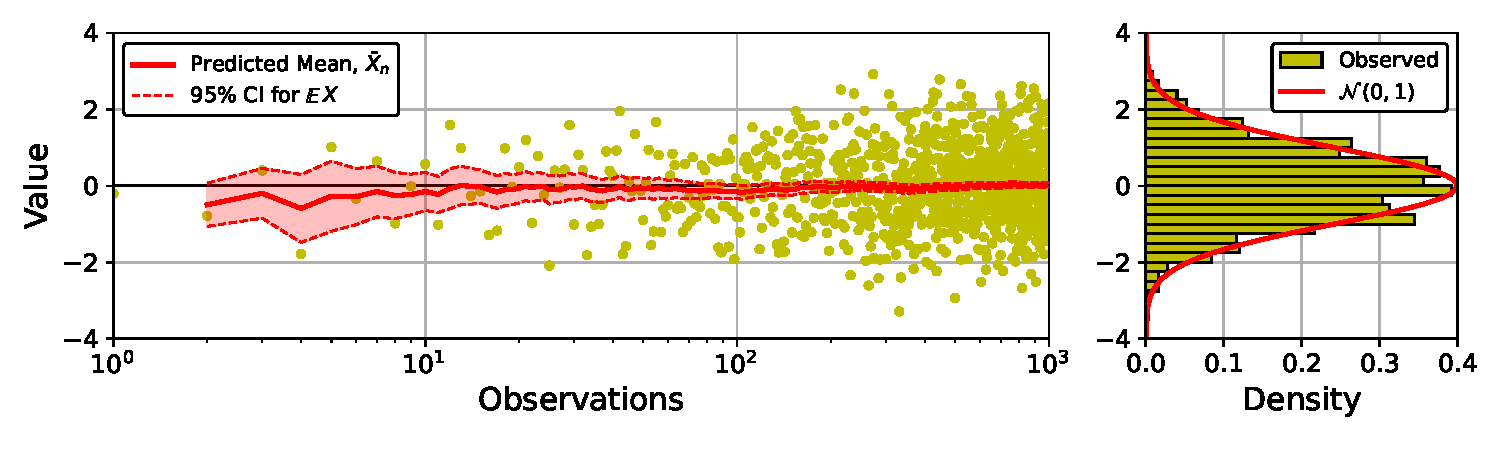
\includegraphics[width=\textwidth]{figures/05a_uncertainty_vs_variability_1000.pdf}
		\end{center}
	\end{frame}

	\begin{frame}
		\frametitle{Uncertainty Quantification in GPR}
		\begin{itemize}
			\item Predictive variance as a measure of confidence in model prediction
			\item For noiseless observations, no distinction: $\V{y}=\V{f(\vect{x})}$
			\item When noise is independent of input $\vect{x}$,
			\begin{equation*}
				\V{y}=\V{f(\vect{x})+\eps}=\V{f(\vect{x})}+\sigma_\eps^2
			\end{equation*}
			\item We can quantify uncertainty ``for the mean'' or ``for outputs.''
		\end{itemize}
	\end{frame}
	
	\subsection{Heteroscedastic GPR}
	\begin{frame}
		\frametitle{What if the Noise Level Varies?}
		\begin{itemize}
			\item Single hyperparameter $\sigma_\eps^2$ implies homoscedasticity.
			\item Estimate $v_i\approx\sigma_\eps^2(\vect{x}_i)$ and use $K_{\vect{y}}=K(X,X)+\diag(\vect{v})$.
			\item For complete results, also need $v_\star\approx\sigma_\eps^2(\vect{x}_\star)$ at test points.
		\end{itemize}
	\end{frame}
	
	\begin{frame}
		\frametitle{GPR with Heteroscedastic Noise}
		\begin{itemize}
			\item Use a secondary GPR to model the varying noise level.
			\item Incorporate noise estimates into likelihood of primary model.
		\end{itemize}
		\vspace{2mm}
	
		\begin{center}
			\includegraphics<1>[scale=0.5]{figures/05b_homoscedastic_GPR.pdf}
			
			\includegraphics<2>[scale=0.5]{figures/05c_heteroscedastic_GPR.pdf}
		\end{center}
		\citeAY{Kersting \emph{et al.}, 2007; Zhang \emph{et al.}, 2020}
	\end{frame}
	
	\subsection{Categorical Inputs}
	\begin{frame}
		\frametitle{GPR with Qualitative Inputs}
		\begin{itemize}
			\item Model a system as $f:\R^d\times S\to\R$ with $S=\{1,2,\ldots,n_s\}$.
			\item Can we do better than $n_s$ separate fits?
			\item If the $n_s$ surfaces are correlated, we can use expanded kernel $$k\left((\vect{x},s),(\vect{x}',s')\right)=C_{s,s'}\tilde{k}(\vect{x},\vect{x}')\,,$$ where $C\in\R^{n_s\times n_s}$ is a cross-correlation matrix.
		\end{itemize}
		\citeAY{Santner \emph{et al.}, 2018}
	\end{frame}
	
	\begin{frame}
		\frametitle{Modeling Cross-Correlation}
		\begin{itemize}
			\item Describe correlation between response surfaces $f(\cdot,s)$.
			\item Must have $C_{s,s}=1$ and $|C_{s,s'}|\leq1$ for all $s,s'\in S$.
			\item Options include:
			\begin{itemize}
				\item Exchangable model:
				\begin{equation*}
					C_{s,s'}=\left\{
					\begin{array}{cl}
						1 & : s=s'\\
						\rho & : s\neq s'
					\end{array}\right.
				\end{equation*}
				\item Toeplitz model for ordinal categories: $C_{s,s'}=e^{-\gamma|s-s'|}$ %\exp\!\left[-\gamma|s-s'|\right]
				\item Specify all $n_s(n_s-1)$ superdiagonal entries.
			\end{itemize}
		\end{itemize}
		\citeAY{Qian \emph{et al.}, 2008; Santner \emph{et al.}, 2018}
	\end{frame}
	
	\begin{frame}
		\frametitle{Mixed-Input Example: \only<1>{Data}\only<2>{Disjoint Fits}\only<3>{Combined Fit}}
		\onslide<1->{
			\begin{equation*}
				f:[-1,1]\times\{1,2\}:(x,s)\mapsto\left\{
				\begin{array}{cl}
					1.9\cos(x-0.15)-0.73 & : s=1\\
					(1-x^2)e^{-x^2} & : s=2
				\end{array}
				\right.
			\end{equation*}
		}
		\begin{center}
			\includegraphics<1>[width=0.9\textwidth]{figures/06b_mixed_data_model.pdf}
			
			\includegraphics<2>[width=0.9\textwidth]{figures/06e_mixed_GPR_disjoint.pdf}
			
			\includegraphics<3>[width=0.9\textwidth]{figures/06d_mixed_GPR_fit.pdf}
		\end{center}
	\end{frame}
	
	\begin{frame}
		\frametitle{Multiple Regression}
		\begin{itemize}
			\item The qualitative input scheme also works for multiple outputs: $$\vect{y}=\mathbf{f}(\vect{x})\in\R^{d'}\;\;\longleftrightarrow\;\; y_s=f(\vect{x},s)$$
			\item Such an approach can accommodate missing output data.
		\end{itemize}
		\begin{center}
			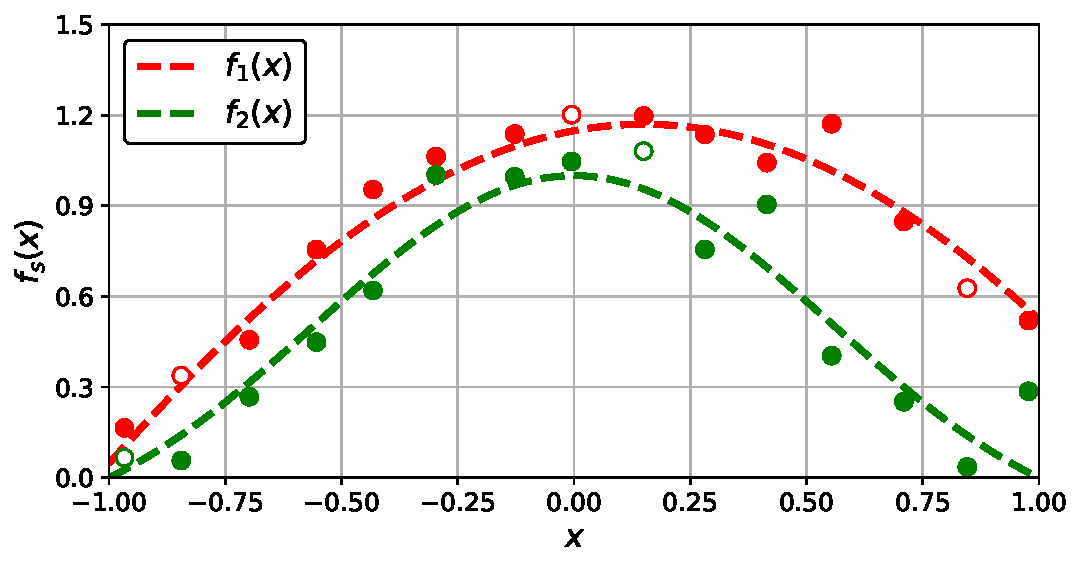
\includegraphics[width=0.9\textwidth]{figures/06f_multiple_regression.pdf}
		\end{center}
		\citeAY{Santner \emph{et al.}, 2018}
	\end{frame}
	
	\section{Bayesian Optimization}
	\subsection{The Algorithm}
	\begin{frame}
		\frametitle{Bayesian Optimization}
		\begin{itemize}
			\item Objective $f:\mathcal{X}\to\R$ on domain $\mathcal{X}\subseteq\R^d$.
			\item We seek a global minimizer $$\vect{x}^\star\in\argminn_{\vect{x}\in\mathcal{X}}f(\vect{x})\,.$$
			\item Bayesian optimization (BO) is most appropriate when:
			\begin{itemize}
				\item Evaluating $f$ is expensive (and possibly noisy).
				\item We have no derivative information.
			\end{itemize}
		\end{itemize}
		\citeAY{Frazier, 2018}
	\end{frame}
	
	\begin{frame}
		\frametitle{Basic BO Algorithm}
		\begin{algorithm}[H]
			\caption{Bayesian Optimization}
			\SetAlgoLined
			\KwData{objective function $f:\mathcal{X}\to\R$; initial sample $\mathcal{D}_n=\{(\vect{x}_i,y_i)\}_{i=1}^n$}
			\For{$i\in\{n+1,\ldots,N\}$}{
				Fit a GPR model to data $\mathcal{D}_{i-1}$\;
				Choose a new point $\vect{x}_i\in\mathcal{X}$\;
				Evaluate $y_i\gets f(\vect{x}_i)$\;
				Update sample $\mathcal{D}_i\gets\mathcal{D}_{i-1}\cup\{(\vect{x}_i,y_i)\}$\;
			}
			$j\gets\argminn_{1\leq i\leq N}y_i$\;
			\KwResult{approximate global minimizer $\vect{x}_j$}
		\end{algorithm}
	\end{frame}

	\begin{frame}
		\frametitle{An Illustrated Example}
		\begin{center}
			\includegraphics<1>[width=\textwidth]{figures/07_example_BO_00.pdf}
			
			\includegraphics<2>[width=\textwidth]{figures/07_example_BO_01.pdf}
			
			\includegraphics<3>[width=\textwidth]{figures/07_example_BO_02.pdf}
			
			\includegraphics<4>[width=\textwidth]{figures/07_example_BO_03.pdf}
			
			\includegraphics<5>[width=\textwidth]{figures/07_example_BO_04.pdf}
			
			\includegraphics<6>[width=\textwidth]{figures/07_example_BO_05.pdf}
			
			\includegraphics<7>[width=\textwidth]{figures/07_example_BO_06.pdf}
			
			\includegraphics<8>[width=\textwidth]{figures/07_example_BO_07.pdf}
			
			\includegraphics<9>[width=\textwidth]{figures/07_example_BO_08.pdf}
			
			\includegraphics<10>[width=\textwidth]{figures/07_example_BO_09.pdf}
			
			\includegraphics<11>[width=\textwidth]{figures/07_example_BO_10.pdf}
			
			\includegraphics<12>[width=\textwidth]{figures/07_example_BO_11.pdf}
			
			\includegraphics<13>[width=\textwidth]{figures/07_example_BO_12.pdf}
		\end{center}
	\end{frame}

	\subsection{Acquisition Functions}
	\begin{frame}
		\frametitle{Selecting the Next Sample Point}
		\begin{itemize}
			\item Use current knowledge to inform our choice.
			\item Exploration vs. Exploitation
			\item An acquisition function measures utility of sampling at $\vect{x}\in\mathcal{X}$: $$\vect{x}_{i+1}=\argmaxx_{\vect{x}\in\mathcal{X}}\alpha(\vect{x};\mathcal{D}_i)$$
			\item How is this better? Optimizing $\alpha$ does not require evaluating $f$.
		\end{itemize}
		\citeAY{Shahriari \emph{et al.}, 2015}
	\end{frame}

	\begin{frame}
		\frametitle{Acquisition Function: Probability of Improvement}
		\begin{itemize}
			\item Which inputs are likely to improve the current best observation?
			\item Gaussian distribution provides an analytical expression: $$\alpha_{PI}(\vect{x};\mathcal{D})=\Pr[f(\vect{x})<\tau\,|\,\mathcal{D}]=\Phi\left(\frac{\tau-\mu(\vect{x})}{\sigma(\vect{x})}\right)$$
			\item Threshold $\tau$ usually written as $\tau=y_{\text{min}}-\delta$ for $\delta\geq0$.
		\end{itemize}
		\begin{center}
			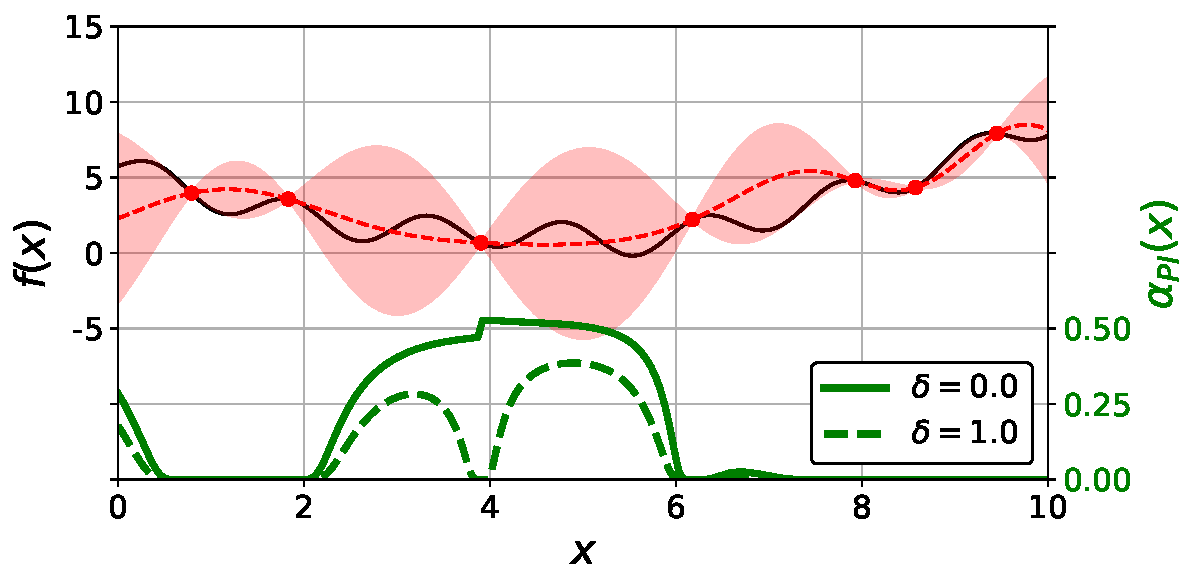
\includegraphics[width=0.8\textwidth]{figures/08a_PI.pdf}
		\end{center}
	\end{frame}
	
	\begin{frame}
		\frametitle{Acquisition Function: Expected Improvement}
		\begin{itemize}
			\item Not all improvements are equally helpful.
			\item Expected improvement compared to threshold $\tau$ is
			\begin{align*}
				\alpha_{EI}(\vect{x};\mathcal{D}) & =\E{\max(0,\,\tau-\nml\left[\mu(\vect{x}),\sigma^2(\vect{x})\right])}\\
				& =(\tau-\mu(\vect{x}))\,\Phi\left(\frac{\tau-\mu(\vect{x})}{\sigma(\vect{x})}\right)+\sigma(\vect{x})\,\phi\left(\frac{\tau-\mu(\vect{x})}{\sigma(\vect{x})}\right)\,.
			\end{align*}
			\item Less prone than PI to become stuck in a local minimum.
		\end{itemize}
		\begin{center}
			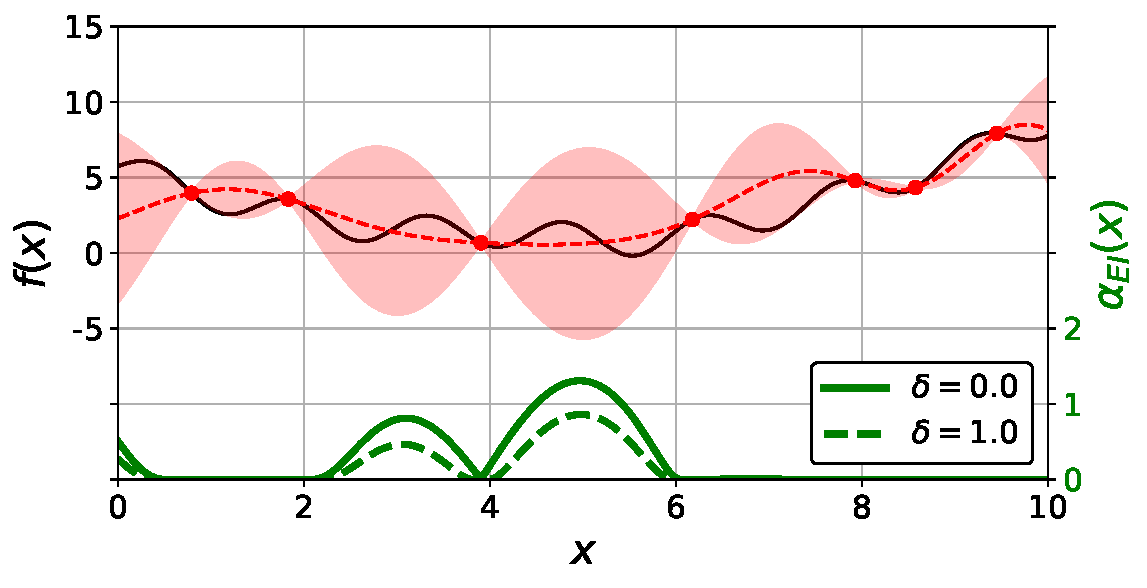
\includegraphics[width=0.8\textwidth]{figures/08b_EI.pdf}
		\end{center}
	\end{frame}
	
	\begin{frame}
		\frametitle{Acquisition Function: Lower Confidence Bound}
		\begin{itemize}
			\item Which inputs have superior best-case outputs?
			\item Usually expressed as a loss to be minimized: $$\alpha_{LCB}(\vect{x};\mathcal{D})=\mu(\vect{x})-\kappa\sigma(\vect{x})\,.$$
		\end{itemize}
		\begin{center}
			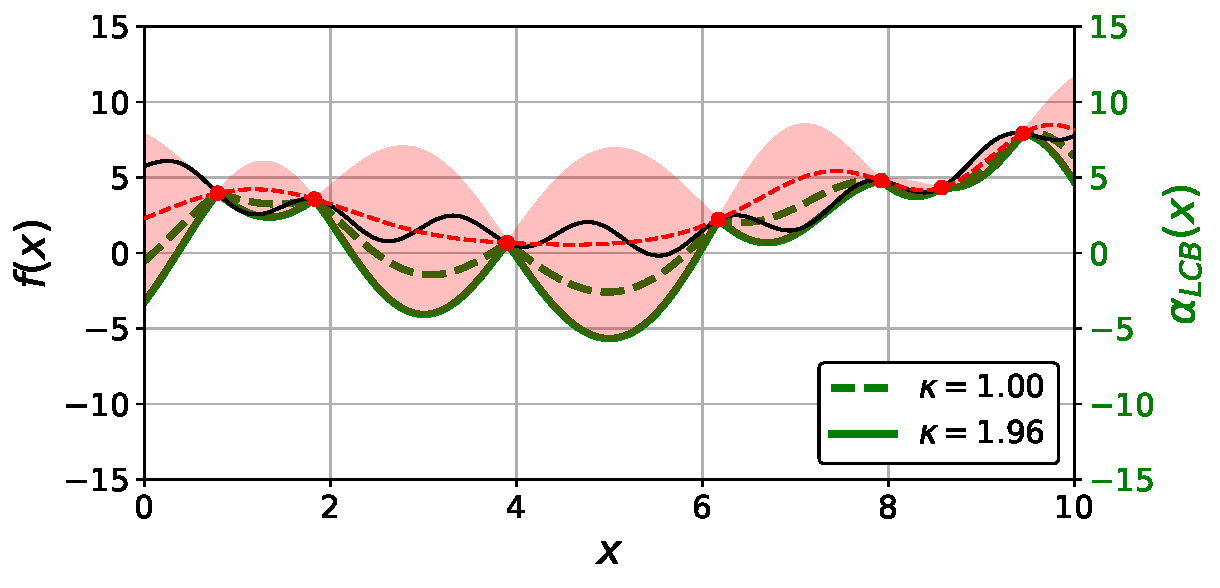
\includegraphics[width=0.8\textwidth]{figures/08c_LCB.pdf}
		\end{center}
	\end{frame}
	
	\subsection{Practical Considerations}
	\begin{frame}
		\frametitle{Computational Cost}
		\begin{itemize}
			\item Inverting $K(X,X)\in\R^{n\times n}$ requires $O(n^3)$ operations.
			\item Cholesky decomposition must be updated each iteration.
			\item Approximation techniques exchange accuracy for speed.
			\item Using a sparse kernel for the GPR may help.
		\end{itemize}
		\citeAY{Duvenaud, 2014; Shahriari \emph{et al.}, 2015}
	\end{frame}
	
	\begin{frame}
		\frametitle{Pre-processing Data}
		\begin{itemize}
			\item Transforming sample data can facilitate GPR performance.
			\begin{itemize}
				\item Normalize observations: $$\tilde{\vect{x}}_i=\frac{\vect{x}_i-\bar{\vect{x}}}{s_x}\qquad\qquad\tilde{y}_i=\frac{y_i-\bar{y}}{s_y}$$
				\item If outputs are necessarily positive: $\tilde{y}_i=\log(y_i)$.
			\end{itemize}
			\item Apply knowledge of problem when deciding how to process data.
			\item Must reverse transformations to recover interpretable quantities.
		\end{itemize}
	\end{frame}

	\begin{frame}
		\frametitle{Generating a Useful Initial Sample}
		\begin{itemize}
			\item Samples drawn uniformly may not fill the domain.
			\item Latin hypercube sampling offers better samples for regression.
		\end{itemize}
		\begin{center}
			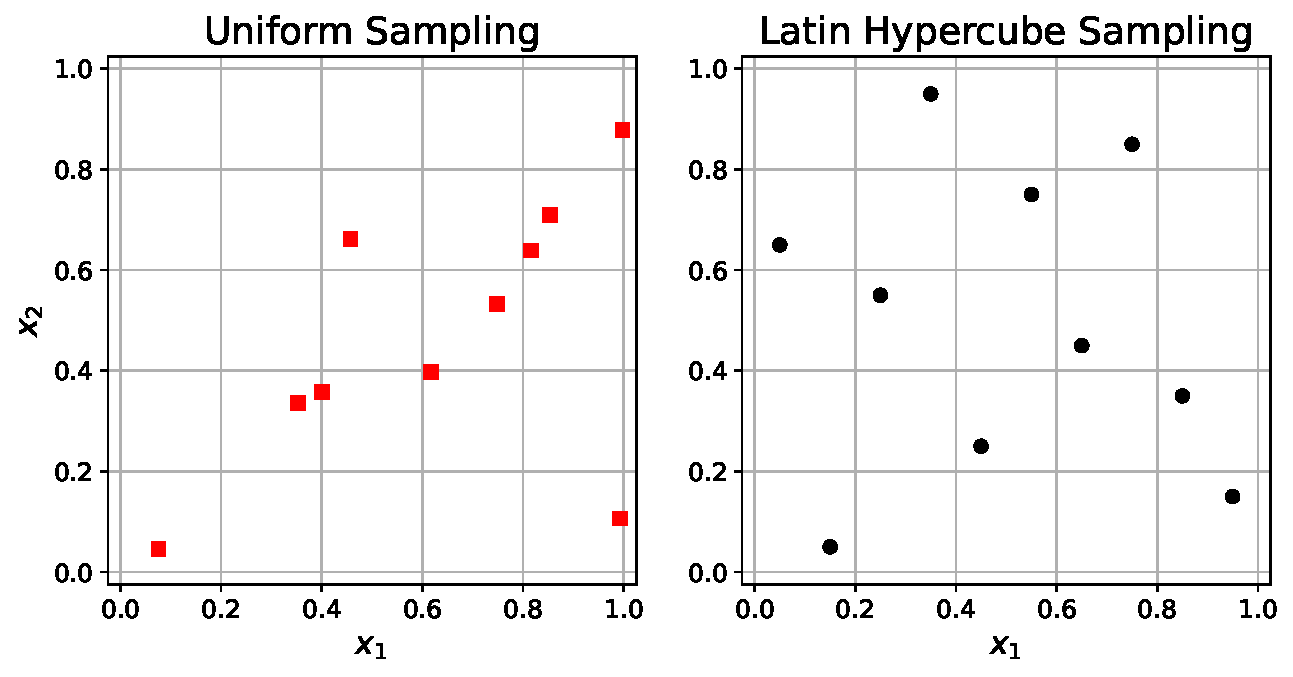
\includegraphics[width=0.8\textwidth]{figures/09_sampling.pdf}
		\end{center}
		\citeAY{Santner \emph{et al.}, 2018}
	\end{frame}
	
	\section{Conclusion}
	\begin{frame}
		\frametitle{Final Thoughts}
		\begin{itemize}
			\item GPs offer a rich environment for mathematical modeling.
			\item Regression is possible without explicit functional forms.
			\item Bayesian framework provides a natural measure of uncertainty.
			\item Expensive optimization problems benefit from efficient sampling.
		\end{itemize}
		\vfill
		\begin{center}
			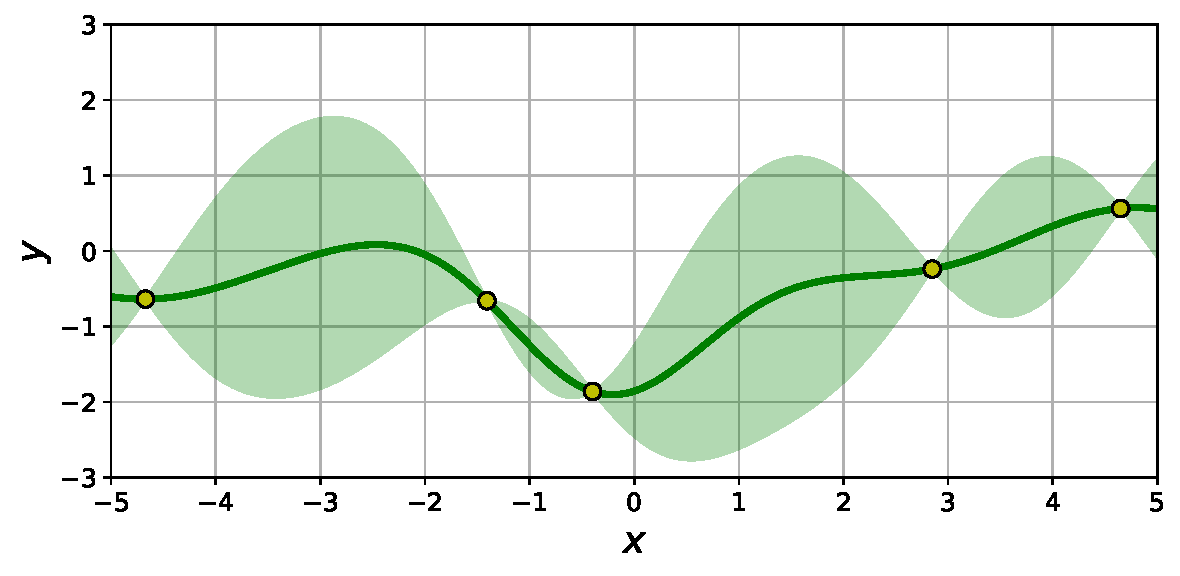
\includegraphics[scale=0.4]{figures/02b_posterior_distribution.pdf}
		\end{center}
	\end{frame}
	
	\begin{frame}[allowframebreaks]
		\frametitle{References}
	\begin{itemize}
			\item Begg, S.H.; Bratvold, R.B.; Welsh, M.B. ``Uncertainty vs. Variability: What’s the Difference and Why is it Important?'' in \emph{Society of Petroleum Engineers Hydrocarbon Economics and Evaluation Symposium}, Houston, TX, \textbf{2014}.
			\item Der Kiureghian, A.; Ditlevsen, O. ``Aleatory or Epistemic? Does it Matter?'' \emph{Struct. Saf.}, 31, 105--112, \textbf{2009}.
			\item Duvenaud, D.K. \emph{Automatic Model Construction with Gaussian Processes} [Ph.D. dissertation], Pembroke College: Cambridge, England, \textbf{2014}.
			\item Frazier, P.I. ``A Tutorial on Bayesian Optimization,'' \emph{arXiv Preprint}, 22 pp., \textbf{2018}. \href{https://arxiv.org/abs/1807.02811}{arXiv:1807.02811}
			\item Goldberg, P.W.; Williams, C.K.I.; Bishop, C.M. ``Regression with Input-Dependent Noise: A Gaussian Process Treatment,'' \emph{Adv. Neural Inf. Process. Syst.}, 10, 493--499, \textbf{1997}.
			\item Kersting, K.; Plagemann, C.; Pfaff, P.; Burgard, W. ``Most Likely Heteroscedastic Gaussian Process Regression,'' \emph{Proc. 24th ICML}, 393--400, \textbf{2007}.
			% \item Mo\v{c}kus, J. ``On Bayesian Methods for Seeking the Extremum,'' in \emph{Optimization Techniques: IFIP Technical Conference}, 400--04, \textbf{1975}.
			\item Pavliotis, G.A. \emph{Stochastic Processes and Applications: Diffusion Processes, the Fokker-Planck and Langevin Equations}, Springer: New~York, NY, \textbf{2014}.
			\item Qian, P.Z.G.; Wu, H.; Wu, C.F.J. ``Gaussian Process Models for Computer Experiments with Qualitative and Quantitative Factors,'' \emph{Technometrics}, 50(3), 383--396, \textbf{2008}.
			\item Rasmussen, C.E.; Williams, C.K.I. \emph{Gaussian Processes for Machine Learning}, MIT Press: Cambridge, MA, \textbf{2006}.
			\item Santner, T.J.; Williams, B.J.; Notz, W.I. \emph{The Design and Analysis of Computer Experiments},'' 2nd ed., Springer: New York, NY, \textbf{2018}.
			\item Shahriari, B.; Swersky, K.; Wang, Z.; Adams, R.P.; de Freitas, N. ``Taking the Human Out of the Loop: A Review of Bayesian Optimization,'' \emph{Proc. IEEE}, 104(1), 148--75, \textbf{2015}.
			\item Zhang, Q.H.; Ni, Y.Q. ``Improved Most Likely Heteroscedastic Gaussian Process Regression via Bayesian Residual Moment Estimator,'' \emph{IEEE Trans. Signal Process.}, 68, 3450--3460, \textbf{2020}.
		\end{itemize}
	\end{frame}
\end{document}
